
%(BEGIN_QUESTION)
% Copyright 2014, Tony R. Kuphaldt, released under the Creative Commons Attribution License (v 1.0)
% This means you may do almost anything with this work of mine, so long as you give me proper credit

Calculate the individual currents through the inductor and through the resistor, the total current, and the total circuit impedance:

$$\includegraphics[width=15.5cm]{i01054x01.eps}$$

Also, draw a phasor diagram showing how the individual component currents relate to the total current.

\underbar{file i01054}
%(END_QUESTION)





%(BEGIN_ANSWER)

$I_L$ = 530.5 $\mu$A RMS

\vskip 10pt

$I_R$ = 490.2 $\mu$A RMS

\vskip 10pt

$I_{total}$ = 722.3 $\mu$A RMS

\vskip 10pt

$Z_{total}$ = 3.461 k$\Omega$

%(END_ANSWER)





%(BEGIN_NOTES)

This would be an excellent question to have students present methods of solution for.  Sometimes I have students present nothing but their solution steps on the board in front of class (no arithmetic at all), in order to generate a discussion on problem-solving strategies.  The important part of their education here is not to arrive at the correct answer or to memorize an algorithm for solving this type of problem, but rather how to {\it think} like a problem-solver, and how to methodically apply the math they know to the problem(s) at hand.


%(END_NOTES)


